\documentclass[aspectratio=169]{beamer}

\usetheme{default}
\setbeamertemplate{navigation symbols}{}
\setbeamertemplate{enumerate item}{\color{navy}\arabic{enumi}.}
\setbeamertemplate{itemize item}{\color{black}\textbullet}
\setbeamertemplate{itemize subitem}{\color{black}\textbullet}
\usepackage{booktabs}
\usepackage{xcolor}
\usepackage{pgfplots}
\pgfplotsset{compat=1.18}
\usepackage{tikz}
\usetikzlibrary{shapes,arrows,positioning}
\usepackage{graphicx}
\definecolor{navy}{RGB}{0, 0, 128}
\definecolor{lightblue}{RGB}{230,240,250}
\definecolor{darkgreen}{RGB}{0,100,0}
\definecolor{lightgreen}{RGB}{230,250,230}
\newcommand{\highlight}[1]{\colorbox{lightblue}{$\displaystyle\textcolor{navy}{#1}$}}
\newcommand{\highlighttext}[1]{\colorbox{lightblue}{\textcolor{navy}{#1}}}
\newcommand{\highlightgreen}[1]{\colorbox{lightgreen}{$\displaystyle\textcolor{darkgreen}{#1}$}}

\usepackage{hyperref}
\hypersetup{
    colorlinks=true,
    linkcolor=navy,
    urlcolor=navy,
    citecolor=navy
}

\begin{document}

\begin{frame}

\textcolor{navy}{Dimensionality reduction} is a common task in data analysis

\bigskip{}

\onslide<2->{
If 3 variables all give the same information, why not just have 1?
}

\bigskip{}

\onslide<3->{
There are two related methods for reducing dimensionality:
\bigskip{}
}

\onslide<4->{
\begin{itemize}
\itemsep1.5em
\item<4-> \textcolor{navy}{Principle Components Analysis (PCA)}
\item<5-> \textcolor{navy}{Factor Analysis}
\end{itemize}
}

\end{frame}

\begin{frame}

PCA is one way to reduce dimensionality. Let $M$ be an $N\times J$ matrix of data

\bigskip{}

\onslide<2->{
Decompose $M$ as follows:
\begin{align*}
\underbrace{M}_{N\times J} &= \underbrace{\boldsymbol{\theta}}_{N\times J} \times \underbrace{\Lambda}_{J\times J}
\end{align*}
}

\onslide<3->{
\begin{itemize}
\itemsep1.5em
\item<3-> $\Lambda$ are stacked eigenvectors
\item<4-> $\boldsymbol{\theta}$ is an \textcolor{navy}{orthogonalized transformation} of $M$ (columns of $\boldsymbol{\theta}$ are independent)
\item<5-> $\Lambda$ indicates the rotation angle to get from $\boldsymbol{\theta}$ back to $M$
\item<6-> If $M$ were orthogonal to begin with, $\Lambda = I$ and $M=\boldsymbol{\theta}$
\end{itemize}
}

\end{frame}

\begin{frame}

Nothing on the previous slide helps us with dimensionality reduction per se

\bigskip{}

\onslide<2->{
\begin{itemize}
\itemsep1.5em
\item<2-> Reduce dimensionality by choosing the largest-magnitude eigenvectors
\item<3-> These represent the dimensions $\boldsymbol{\theta}$ with the greatest variance
\item<4-> We say that we ``select the first $K$ \textcolor{navy}{principal components} of $M$''
\end{itemize}
}

\end{frame}

\begin{frame}

Mathematically, we ``reduce'' (i.e.\ ``approximate'') $M$ by choosing a subset of $\boldsymbol{\theta}$ and $\Lambda$

\bigskip{}

\onslide<2->{
\begin{align*}
\underbrace{\widetilde{M}}_{N\times J} &= \underbrace{\boldsymbol{\theta}_k}_{N\times K} \times \underbrace{\Lambda_{k}^{'}}_{K\times J}
\end{align*}

}

\bigskip{}

\onslide<3->{
\begin{align*}
M &= \boldsymbol{\theta}_k\Lambda_{k}^{'} + \boldsymbol{\varepsilon}
\end{align*}
}

\onslide<4->{
where $\boldsymbol{\varepsilon}\equiv M - \widetilde{M}$ is a $N\times J$ matrix
}

\end{frame}

\begin{frame}

\begin{center}
\begin{tikzpicture}

\only<1-2>{
% Before transformation (left plot)
\begin{axis}[
    name=before,
    width=8.5cm,
    height=8.5cm,
    xmin=-4, xmax=4,
    ymin=-4, ymax=4,
    grid=major,
    grid style={dotted, gray!30},
    xlabel={$x_1$},
    ylabel={$x_2$},
    % title={Original Basis},
    % title style={font=\large\bfseries},
    axis equal,
]

% Data points (visible on all overlays)
\addplot[
    only marks,
    mark=*,
    mark size=1.5pt,
    blue!70!black,
    opacity=0.6,
] coordinates {
(-0.5382, -0.5219) ( 0.8672,  1.2193) ( 0.9760,  0.5437) ( 0.3374,  0.1930) (-0.9961, -0.7397) (-0.5232, -1.2720) (-1.2974, -2.0238) ( 0.9174,  0.5173) ( 0.1766, -0.6455) ( 0.7552,  1.5121) (-0.5915, -0.2270) ( 1.8444,  1.9488) ( 1.8169,  2.3597) (-0.1238,  0.1905) (-1.1106, -1.5477) (-0.6809,  0.2780) ( 0.0142,  0.0629) (-0.0596,  0.1939) (-0.6610, -0.1486) ( 0.3060, -0.1580) (-0.4091, -0.8537) (-1.2819, -1.7735) (-0.2849, -0.3006) (-0.0648,  0.3696) ( 1.0004,  0.5430) (-0.8013, -0.7842) ( 0.0918, -0.0333) ( 0.2738, -0.2550) (-2.1335, -2.5641) ( 0.4040,  0.2272) (-0.9585, -0.5437) (-0.3263, -0.5107) ( 2.4787,  2.5095) ( 1.5391,  1.8181) ( 0.8270,  0.7388) (-0.1596,  0.3645) (-0.8577, -0.3508) ( 0.3984, -0.0760) (-0.2248, -0.2302) (-1.3147, -1.4904) (-0.0218, -0.8632) (-0.8801, -1.4047) ( 1.1086,  1.4535) (-0.4641, -0.4604) ( 0.6646,  0.4361) (-0.5301, -0.8120) ( 0.0409,  0.7693) ( 0.1551, -0.3341) (-0.3211, -0.8857) ( 2.1458,  2.1305) ( 0.8004,  1.5928) ( 1.1963,  0.7571) ( 2.0975,  2.2182) ( 0.3877,  0.7315) ( 1.0453,  0.7617) (-1.3718, -0.8774) (-0.9584, -1.1552) (-2.6689, -2.2423) (-0.8027, -0.6201) (-0.4510, -0.3719) (-0.7366, -1.6198) ( 1.1147,  1.4137) (-0.8534, -1.1322) (-0.7588, -1.3579) ( 0.0980, -0.9757) (-0.8496, -0.7370) ( 0.5607,  0.7459) (-0.3475, -1.2878) ( 1.3709,  1.3973) ( 0.7410,  0.3909) (-0.7129, -0.6041) ( 0.8047, -0.0851) ( 0.9776,  1.2375) ( 0.9396,  0.7618) (-2.2629, -1.2706) (-0.5137, -1.1886) (-1.9895, -2.3070) ( 1.6782,  1.2842) ( 0.3587,  1.0428) (-0.2533,  0.4678) (-1.1469, -1.4030) (-0.7009, -0.5497) (-0.6454,  0.3775) ( 0.7819,  0.8685) ( 0.3157,  0.3488) ( 1.2744,  0.2649) (-0.0745, -1.2865) (-2.3036, -1.6527) ( 0.9856,  1.9573) ( 1.0236,  1.1539) ( 0.1316, -0.0543) ( 0.6021,  0.3126) (-0.0068,  0.5124) ( 0.0880,  1.0165) (-0.1150,  0.4170) (-1.3616, -0.6733) (-0.7868, -0.4586) (-2.3368, -3.4621) ( 0.4078, -0.3109) (-0.6136,  0.1253) 
};

% Principal component axes (visible from slide 2 onwards)
\only<2>{
\draw[->, line width=2pt, red!70!black] (axis cs:0,0) -- (axis cs:2,2) 
    node[below right, font=\small] {PC1};
\draw[->, line width=2pt, green!50!black] (axis cs:0,0) -- (axis cs:-0.75,0.75) 
    node[above left, font=\small] {PC2};
}

\end{axis}
}

% After transformation (right plot) - visible only on slide 3
\only<3>{
\begin{axis}[
    name=after,
    at={(before.east)},
    anchor=west,
    xshift=1.5cm,
    width=8.5cm,
    height=8.5cm,
    xmin=-4, xmax=4,
    ymin=-4, ymax=4,
    grid=major,
    grid style={dotted, gray!30},
    xlabel={PC1},
    ylabel={PC2},
    % title={Principal Component Basis},
    % title style={font=\large\bfseries},
    axis equal,
]

% Transformed data points
\addplot[
    only marks,
    mark=*,
    mark size=1.5pt,
    blue!70!black,
    opacity=0.6,
] coordinates {
(-0.6668,  0.0705) ( 1.5684,  0.1736) ( 1.1349, -0.3559) ( 0.4490, -0.1106) (-1.1336,  0.2686) (-1.2182, -0.4383) (-2.2944, -0.3576) ( 1.0764, -0.3296) (-0.2852, -0.5465) ( 1.7132,  0.4517) (-0.4815,  0.3059) ( 2.7625, -0.0738) ( 3.0518,  0.2194) ( 0.1411,  0.2328) (-1.8141, -0.1816) (-0.1629,  0.7078) ( 0.1372,  0.0450) ( 0.1863,  0.1870) (-0.4690,  0.4099) ( 0.1654, -0.3199) (-0.8295, -0.2463) (-2.0967, -0.2032) (-0.3332,  0.0277) ( 0.3143,  0.3075) ( 1.1506, -0.3746) (-1.0376,  0.0934) ( 0.1167, -0.0770) ( 0.0715, -0.3602) (-3.2533, -0.0904) ( 0.5187, -0.1378) (-0.9620,  0.3705) (-0.5179, -0.0807) ( 3.6028, -0.1765) ( 2.4622,  0.0680) ( 1.1822, -0.1150) ( 0.2477,  0.3751) (-0.7508,  0.4230) ( 0.2880, -0.3347) (-0.2406,  0.0294) (-1.9067,  0.0091) (-0.5798, -0.5424) (-1.5543, -0.2593) ( 1.9038,  0.1483) (-0.5717,  0.0558) ( 0.8479, -0.1942) (-0.8786, -0.1280) ( 0.6835,  0.4935) (-0.0665, -0.3238) (-0.7951, -0.3334) ( 3.0984, -0.1788) ( 1.8036,  0.4714) ( 1.4408, -0.3792) ( 3.1320, -0.0846) ( 0.8853,  0.2089) ( 1.3441, -0.2632) (-1.4858,  0.4585) (-1.4195, -0.0352) (-3.3676,  0.5238) (-0.9157,  0.2032) (-0.4968,  0.1047) (-1.6201, -0.5094) ( 1.8781,  0.1174) (-1.3326, -0.0985) (-1.4387, -0.3190) (-0.5845, -0.7067) (-1.0344,  0.1608) ( 1.0108,  0.0890) (-1.1135, -0.5803) ( 2.0357, -0.0852) ( 0.8648, -0.2814) (-0.8443,  0.1466) ( 0.5508, -0.6448) ( 1.6552,  0.1031) ( 1.2740, -0.1840) (-2.3712,  0.8645) (-1.1495, -0.3902) (-2.9654, -0.0276) ( 2.1549, -0.3902) ( 1.0990,  0.4371) ( 0.2628,  0.5137) (-1.7300, -0.0586) (-0.7955,  0.1737) (-0.0649,  0.7472) ( 1.2493,  0.0048) ( 0.5511,  0.0090) ( 1.1242, -0.7642) (-0.9315, -0.7837) (-2.6841,  0.6415) ( 2.1991,  0.5745) ( 1.6231,  0.0132) ( 0.1274, -0.1206) ( 0.7140, -0.2294) ( 0.4596,  0.3588) ( 0.8998,  0.6222) ( 0.3165,  0.3765) (-1.3263,  0.5862) (-0.7843,  0.2985) (-4.0602, -0.5338) ( 0.1186, -0.4976) (-0.2325,  0.5561) 
};

% New axes aligned with principal components
\draw[->, line width=2pt, red!70!black] (axis cs:0,0) -- (axis cs:2.8284,0);
\draw[->, line width=2pt, green!50!black] (axis cs:0,0) -- (axis cs:0,1.06066);

\end{axis}
}

% After transformation (right plot) - visible only on slide 3
\only<4>{
\begin{axis}[
    name=after,
    at={(before.east)},
    anchor=west,
    xshift=1.5cm,
    width=8.5cm,
    height=8.5cm,
    xmin=-4, xmax=4,
    ymin=-4, ymax=4,
    grid=major,
    grid style={dotted, gray!30},
    xlabel={PC1},
    ylabel={PC2 (discarded)},
    % title={Principal Component Basis},
    % title style={font=\large\bfseries},
    axis equal,
]

\addplot[
    only marks,
    mark=*,
    mark size=1.5pt,
    red!70!black,
    opacity=0.1,
] coordinates {
(-0.6668,  0.0705) ( 1.5684,  0.1736) ( 1.1349, -0.3559) ( 0.4490, -0.1106) (-1.1336,  0.2686) (-1.2182, -0.4383) (-2.2944, -0.3576) ( 1.0764, -0.3296) (-0.2852, -0.5465) ( 1.7132,  0.4517) (-0.4815,  0.3059) ( 2.7625, -0.0738) ( 3.0518,  0.2194) ( 0.1411,  0.2328) (-1.8141, -0.1816) (-0.1629,  0.7078) ( 0.1372,  0.0450) ( 0.1863,  0.1870) (-0.4690,  0.4099) ( 0.1654, -0.3199) (-0.8295, -0.2463) (-2.0967, -0.2032) (-0.3332,  0.0277) ( 0.3143,  0.3075) ( 1.1506, -0.3746) (-1.0376,  0.0934) ( 0.1167, -0.0770) ( 0.0715, -0.3602) (-3.2533, -0.0904) ( 0.5187, -0.1378) (-0.9620,  0.3705) (-0.5179, -0.0807) ( 3.6028, -0.1765) ( 2.4622,  0.0680) ( 1.1822, -0.1150) ( 0.2477,  0.3751) (-0.7508,  0.4230) ( 0.2880, -0.3347) (-0.2406,  0.0294) (-1.9067,  0.0091) (-0.5798, -0.5424) (-1.5543, -0.2593) ( 1.9038,  0.1483) (-0.5717,  0.0558) ( 0.8479, -0.1942) (-0.8786, -0.1280) ( 0.6835,  0.4935) (-0.0665, -0.3238) (-0.7951, -0.3334) ( 3.0984, -0.1788) ( 1.8036,  0.4714) ( 1.4408, -0.3792) ( 3.1320, -0.0846) ( 0.8853,  0.2089) ( 1.3441, -0.2632) (-1.4858,  0.4585) (-1.4195, -0.0352) (-3.3676,  0.5238) (-0.9157,  0.2032) (-0.4968,  0.1047) (-1.6201, -0.5094) ( 1.8781,  0.1174) (-1.3326, -0.0985) (-1.4387, -0.3190) (-0.5845, -0.7067) (-1.0344,  0.1608) ( 1.0108,  0.0890) (-1.1135, -0.5803) ( 2.0357, -0.0852) ( 0.8648, -0.2814) (-0.8443,  0.1466) ( 0.5508, -0.6448) ( 1.6552,  0.1031) ( 1.2740, -0.1840) (-2.3712,  0.8645) (-1.1495, -0.3902) (-2.9654, -0.0276) ( 2.1549, -0.3902) ( 1.0990,  0.4371) ( 0.2628,  0.5137) (-1.7300, -0.0586) (-0.7955,  0.1737) (-0.0649,  0.7472) ( 1.2493,  0.0048) ( 0.5511,  0.0090) ( 1.1242, -0.7642) (-0.9315, -0.7837) (-2.6841,  0.6415) ( 2.1991,  0.5745) ( 1.6231,  0.0132) ( 0.1274, -0.1206) ( 0.7140, -0.2294) ( 0.4596,  0.3588) ( 0.8998,  0.6222) ( 0.3165,  0.3765) (-1.3263,  0.5862) (-0.7843,  0.2985) (-4.0602, -0.5338) ( 0.1186, -0.4976) (-0.2325,  0.5561) 
};

% Transformed data points
\addplot[
    only marks,
    mark=*,
    mark size=1.5pt,
    blue!70!black,
    opacity=0.6,
] coordinates {
(-0.6668, 0) ( 1.5684, 0) ( 1.1349, 0) ( 0.4490, 0) (-1.1336, 0) (-1.2182, 0) (-2.2944, 0) ( 1.0764, 0) (-0.2852, 0) ( 1.7132, 0) (-0.4815, 0) ( 2.7625, 0) ( 3.0518, 0) ( 0.1411, 0) (-1.8141, 0) (-0.1629, 0) ( 0.1372, 0) ( 0.1863, 0) (-0.4690, 0) ( 0.1654, 0) (-0.8295, 0) (-2.0967, 0) (-0.3332, 0) ( 0.3143, 0) ( 1.1506, 0) (-1.0376, 0) ( 0.1167, 0) ( 0.0715, 0) (-3.2533, 0) ( 0.5187, 0) (-0.9620, 0) (-0.5179, 0) ( 3.6028, 0) ( 2.4622, 0) ( 1.1822, 0) ( 0.2477, 0) (-0.7508, 0) ( 0.2880, 0) (-0.2406, 0) (-1.9067, 0) (-0.5798, 0) (-1.5543, 0) ( 1.9038, 0) (-0.5717, 0) ( 0.8479, 0) (-0.8786, 0) ( 0.6835, 0) (-0.0665, 0) (-0.7951, 0) ( 3.0984, 0) ( 1.8036, 0) ( 1.4408, 0) ( 3.1320, 0) ( 0.8853, 0) ( 1.3441, 0) (-1.4858, 0) (-1.4195, 0) (-3.3676, 0) (-0.9157, 0) (-0.4968, 0) (-1.6201, 0) ( 1.8781, 0) (-1.3326, 0) (-1.4387, 0) (-0.5845, 0) (-1.0344, 0) ( 1.0108, 0) (-1.1135, 0) ( 2.0357, 0) ( 0.8648, 0) (-0.8443, 0) ( 0.5508, 0) ( 1.6552, 0) ( 1.2740, 0) (-2.3712, 0) (-1.1495, 0) (-2.9654, 0) ( 2.1549, 0) ( 1.0990, 0) ( 0.2628, 0) (-1.7300, 0) (-0.7955, 0) (-0.0649, 0) ( 1.2493, 0) ( 0.5511, 0) ( 1.1242, 0) (-0.9315, 0) (-2.6841, 0) ( 2.1991, 0) ( 1.6231, 0) ( 0.1274, 0) ( 0.7140, 0) ( 0.4596, 0) ( 0.8998, 0) ( 0.3165, 0) (-1.3263, 0) (-0.7843, 0) (-4.0602, 0) ( 0.1186, 0) (-0.2325, 0)
};

\end{axis}
}
\end{tikzpicture}
\end{center}

% \vspace{0.5cm}
% \only<1>{Step 1: Original correlated data in $(x_1, x_2)$ basis}
% \only<2>{Step 2: Principal components show directions of maximum variance}
% \only<3>{Step 3: Data transformed to orthogonal PC basis (decorrelated)}
% \bigskip\par
\vspace{-0.5cm}
\only<4>{Use $PC1$ for all further analysis}

\end{frame}

\end{document}